\documentclass{standalone}
\usepackage{tikz}
\usepackage{amsmath,dsfont,bm}
\usetikzlibrary{arrows.meta, positioning, shapes.geometric, calc,patterns,quotes,decorations.pathreplacing}
\newcommand \thetaV {\bm{\theta}^{V}}
\begin{document}
	
	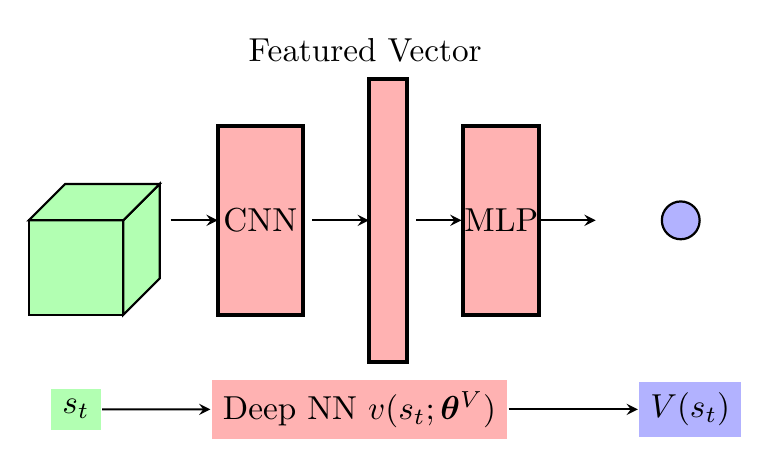
\begin{tikzpicture}[
		thick,scale=1.2, every node/.style={scale=1.2},
		state/.style={draw,circle,pattern=north east lines, pattern color=yellow,radius=0.2},
		action/.style={draw,rectangle, ,pattern=north west lines, pattern color=green}
		]
		
		% Input node (dashed ellipse)
		\pgfmathsetmacro{\cubex}{1}
		\pgfmathsetmacro{\cubey}{1}
		\pgfmathsetmacro{\cubez}{1}
		\draw[black,fill=green!30] (-2,0,0) -- ++(-\cubex,0,0) -- ++(0,-\cubey,0) -- ++(\cubex,0,0) -- cycle;
		\draw[black,fill=green!30] (-2,0,0) -- ++(0,0,-\cubez) -- ++(0,-\cubey,0) -- ++(0,0,\cubez) -- cycle;
		\draw[black,fill=green!30] (-2,0,0) -- ++(-\cubex,0,0) -- ++(0,0,-\cubez) -- ++(\cubex,0,0) -- cycle;
		
		
		% Hidden layers (rectangles)
		\draw[fill=red!30,line width=0.5mm] (-1,1) rectangle (-0.1,-1) node[pos=.5] {CNN};
		\draw[fill=red!30,line width=0.5mm] (0.6,1.5) rectangle (1,-1.5) node[pos=-0.1] {Featured Vector};
		\draw[fill=red!30,line width=0.5mm] (1.6,1) rectangle (2.4,-1) node[pos = 0.5]{MLP};
		
		% Arrows between layers
		\draw[->,>=stealth,thick] (-1.5,0) -- (-1,0);
		\draw[->,>=stealth,thick] (-0,0) -- (0.6,0);
		\draw[->,>=stealth,thick] (1.1,0) -- (1.58,0);
		\draw[->,>=stealth,thick] (2.4,0) -- (3,0);
		
		
		
		% Dotted line between layers
	%	\draw[dotted,thick] (0,0) -- (1,0);
		
		% Output arrows
	%	\foreach \y in {1.0, 0.5, -0.5, -1.0}
	%	\draw[->,>=stealth,thick] (3,0) -- (3.5,0);
		
		% Output circles
	%	\foreach \y in {1.0, 0.5, -0.5, -1.0}
		\filldraw[fill=blue!30] (3.9,0) circle [radius=0.2];
		
		% Output label
	%	\node at (3.9, 0.1) {$\vdots$};
	%	\draw [thick, decorate,decoration={brace,amplitude=10pt},yshift=2pt] (4.1,1.5) -- (4.1,-1.5) node [black,midway,xshift = 18pt,yshift=3pt] {$|\mathds{A}|$};
		
		% Network label
		\node [fill = green!30]at (-2.5,-2) (st){$s_t$};
		
		\node [fill = red!30!]at (0.5, -2)(NN) {Deep NN $v(s_t;\thetaV)$};
		
		% Q-function label
		\node [fill = blue!30] at (4, -2)(Q) {$V(s_t)$};
		\draw[->,>=stealth,thick](st)--(NN);
		\draw[->,>=stealth,thick](NN.east)--(Q.west);
	\end{tikzpicture}
	
\end{document}
